\chapter{C-AD Guidance}
\label{chap:cad}

For planning purposes in this document, we use luminosity projection numbers provided by the C-AD.   The version of the document titled 
``RHIC Collider Projections (FY 2017 –- FY 2027)'' utilized for this study is dated 21 August 2020 and utilizes knowledge gained from the Run-15 p+p and p+Au at 200~GeV running and the Run-16 \auau at 200 GeV running.   The document is available at:

\bigskip
{\color{blue}{http://www.rhichome.bnl.gov/RHIC/Runs/RhicProjections.pdf}} 
\bigskip

The document linked above is periodically updated, so note the date tag.  In general, C-AD provides a minimum and maximum luminosity per week for each running period, as well as the fraction of collisions within a given z-vertex range. For calculating the integrated luminosity, we assume a ramp-up curve and then a steady-state physics running at the mean of the minimum and maximum in both luminosity and z-vertex fraction within $|z|<$10~cm (where a minimum and maximum are given).  The C-AD minimum and maximum projections are fully detailed in the document linked above.

\section{Crossing Angle}

The original C-AD projections for \auau 200~GeV collision rate as a function of time-in-store for the years 2023, 2025, and 2027 are shown in Figure~\ref{fig:auaulumcurves2} (left).    The black curves are the collision rate for interactions at any longitudinal $z$ vertex position, while the red curves are the collision rate for interactions with $|z|<$10~cm.    The magenta curve corresponds to the design specified 15~kHz sPHENIX Level-1 trigger accept rate.
These projections are with zero crossing angle between the beams.   

The sPHENIX optimal acceptance for the inner tracking detectors is with collisions within $|z|<$10~cm.   Thus, it is clear that a majority of the collisions in this running mode with zero crossing angle have highly sub-optimal tracking acceptance.   In principle these collisions far outside the optimal region (i.e. $|z| > 10$~cm) still could be used for calorimeter-only physics measurements (e.g. high $p_{T}$ photons and calorimetric jets) -- however, one would not have good acceptance to measure jet fragmentation functions, or medium response via tracks in these events.    There is a significant down side to the very large collision rate outside of $|z|<$10~cm.   These collisions still leave hits in the TPC and thus substantially increase ion back-flow (IBF) and fluctuations in the IBF.   This additional charge is corrected for but at the same time gets more and more challenging and eventually degrades the track momentum resolution and track finding efficiency.    Additionally, components of sPHENIX including the calorimeter silicon photo-multipliers (SiPMs) are susceptible to radiation damage over time.   These additional collisions significantly increase the overall time-integrated radiation load on the detector.

Therefore, after detailed discussions with C-AD, sPHENIX plans to run with a nominal beam crossing angle of 2 milliradians in \auau collisions.    C-AD has included collision rate information at beam crossing angles of 0, 1, and 2 milliradians in their projections document.    Figure~\ref{fig:auaulumcurves2} (right) shows the collision rate as a function of time in store for a nominal 2 milliradian crossing angle.   There is a modest reduction in collision rate within $|z|<$10~cm; however, it still exceeds the 15~kHz Level-1 accept rate throughout the store.   What is most noticeable is the reduction by almost a factor of three in total collision rate.   This effectively translates into a factor of three lower radiation load on the detector and three times lower charge deposition in the TPC.   Small optimizations around the 2 milliradian value may be possible; for the purposes of this document we have consistently used this 2 milliradian crossing angle for all projections.

\begin{figure}
\centering
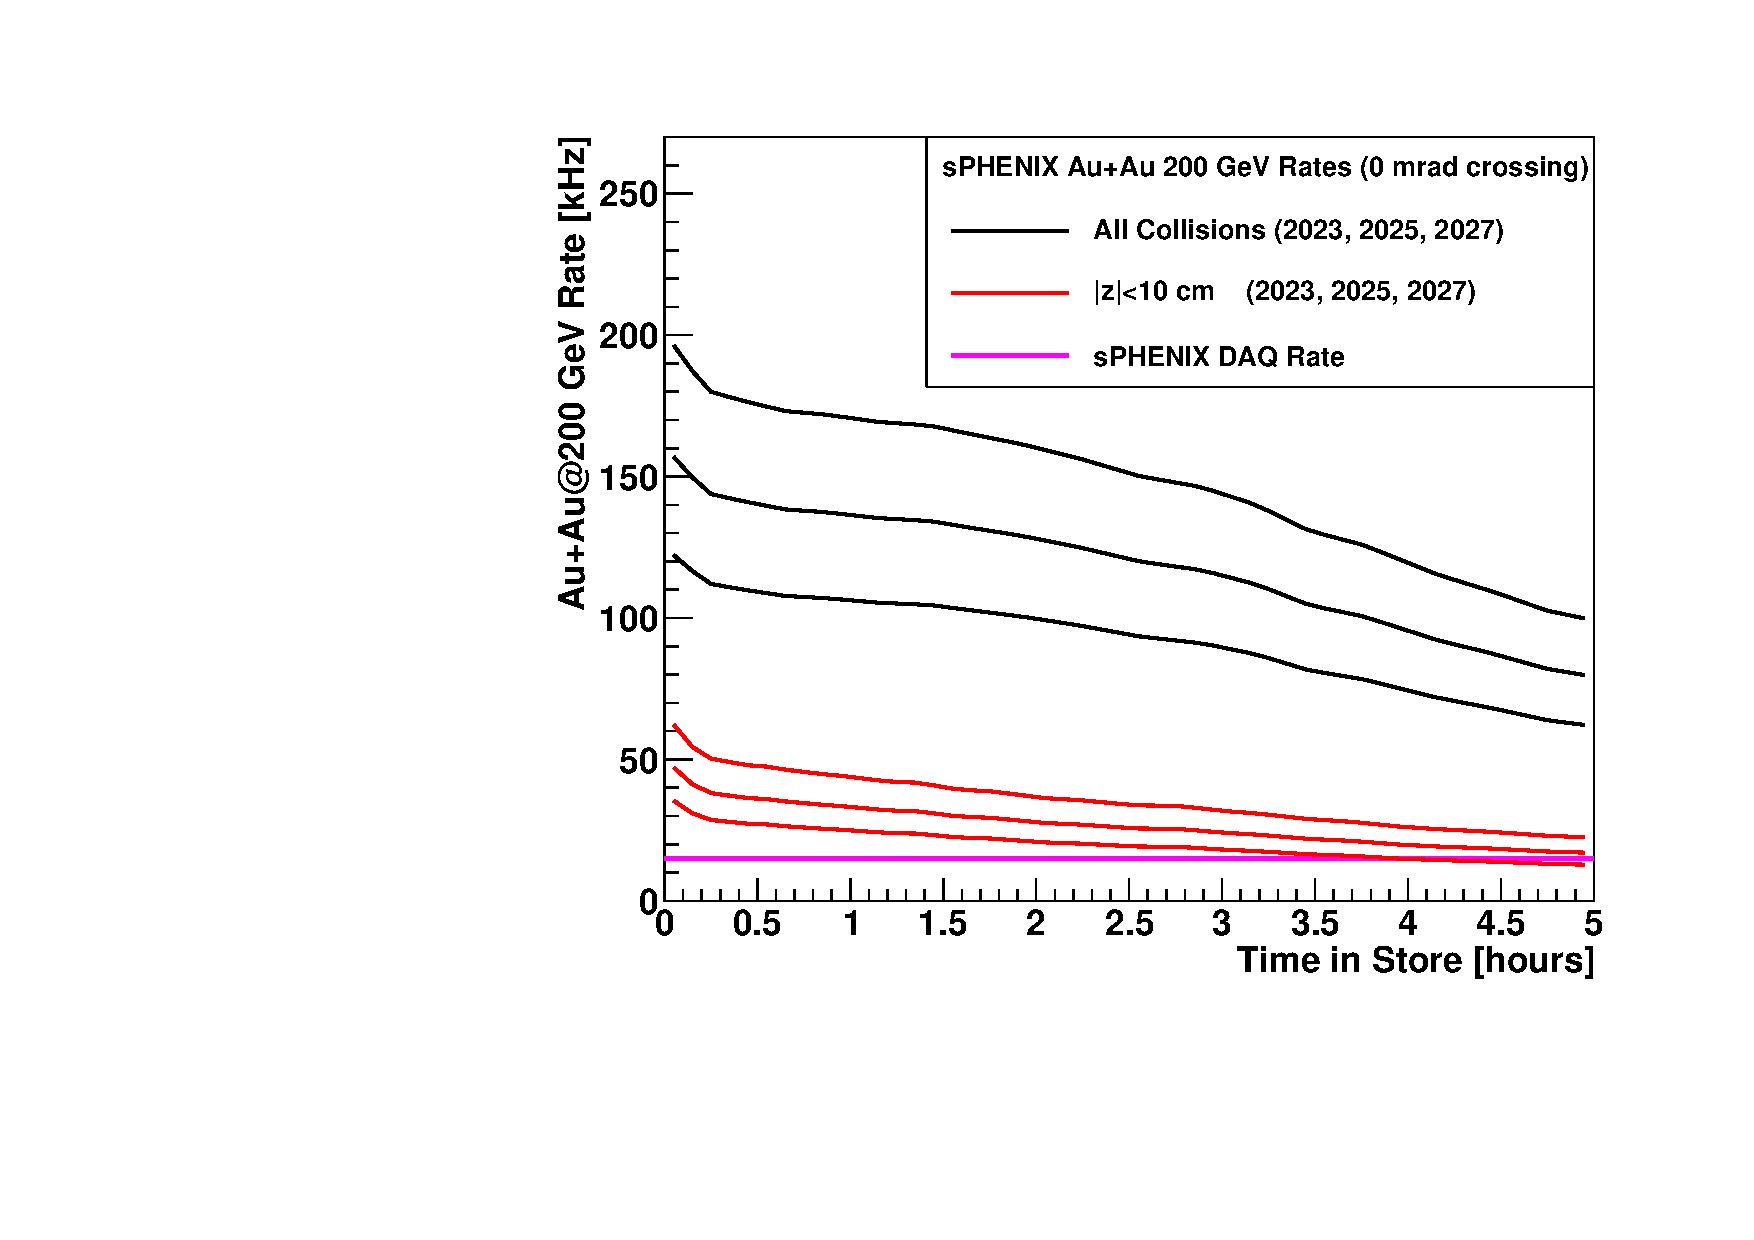
\includegraphics[width=0.47\textwidth]{figs/figure_auauratestore_0mrad.pdf}
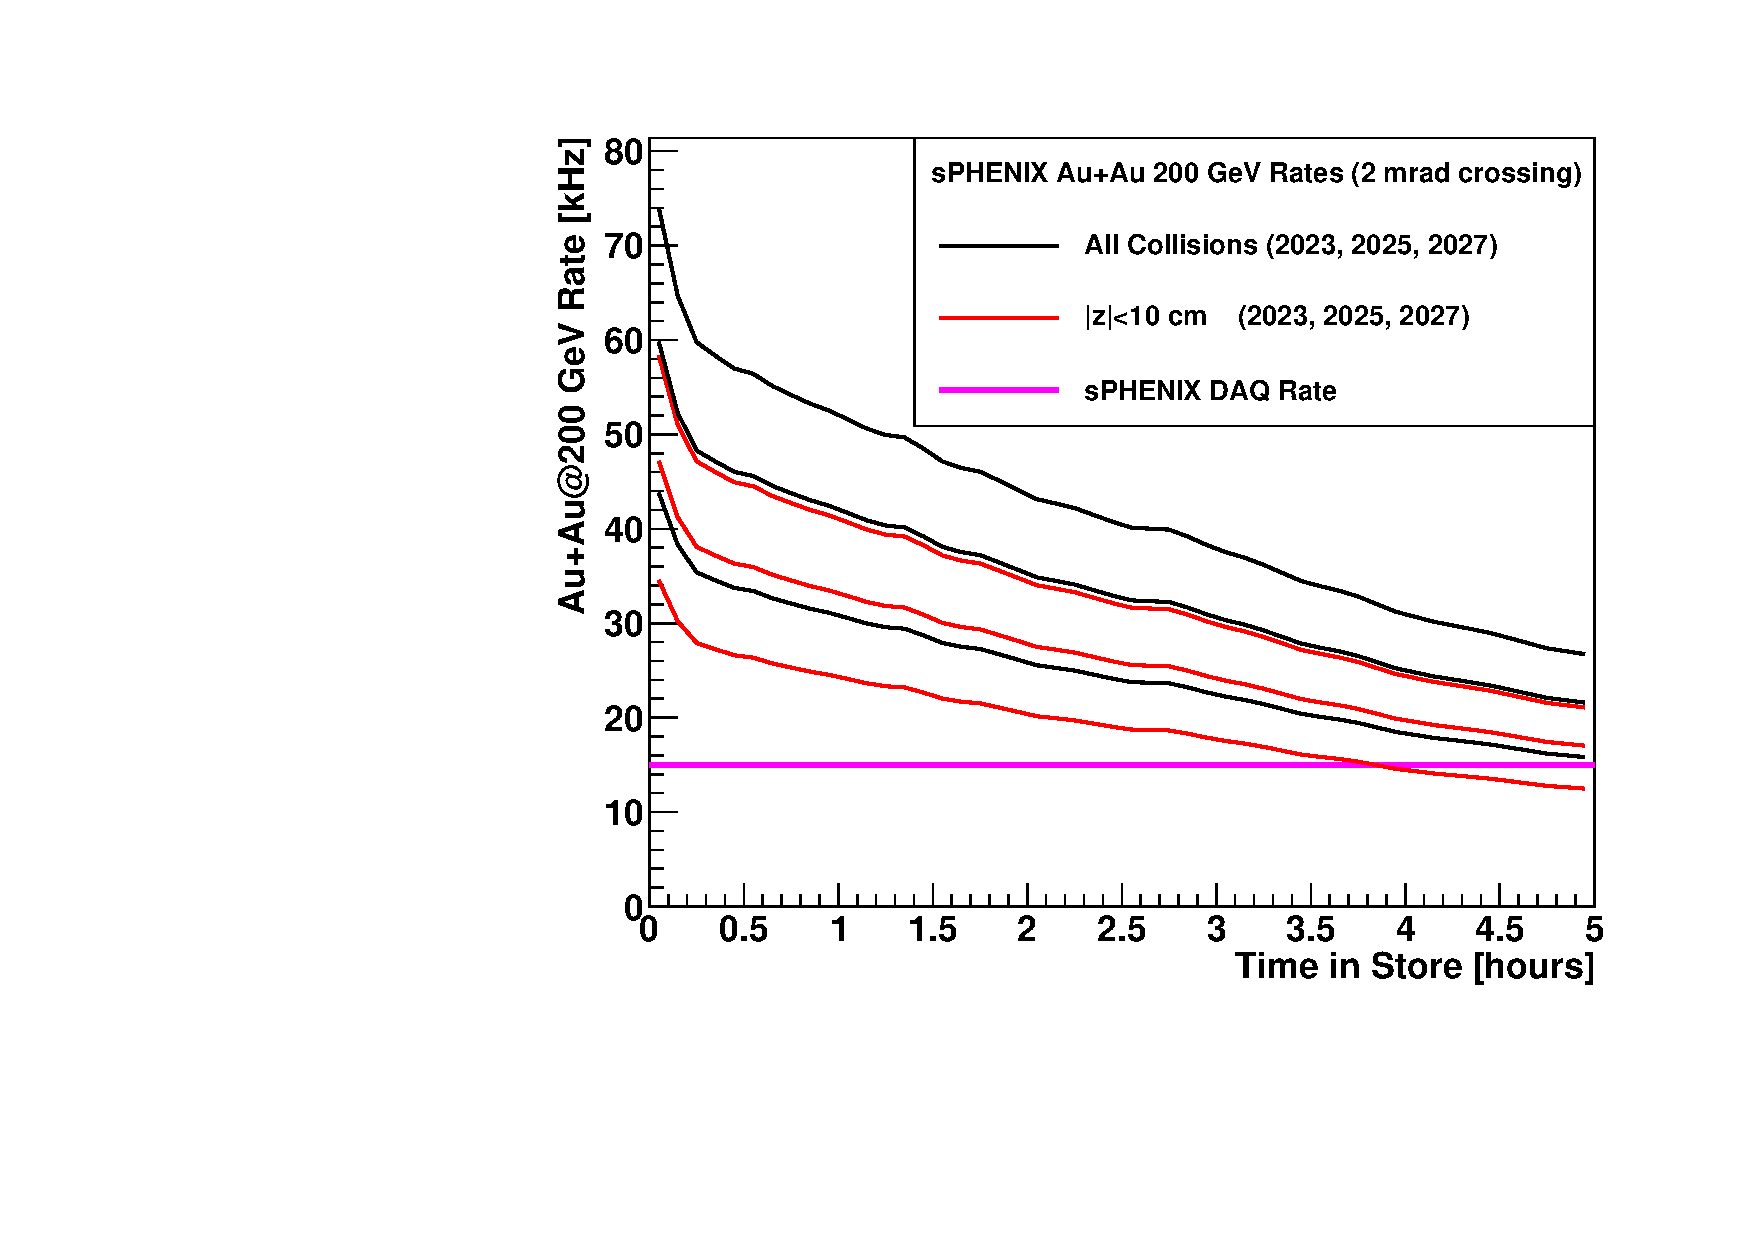
\includegraphics[width=0.47\linewidth]{figs/figure_auauratestore_2mrad.pdf}
\caption{(left) Estimated \auau at 200~GeV collision rate as a function of Time in Store for all collisions (black) and collisions within $\pm$ 10 cm (red).   The bottom to top set of curves in each color are for the C-AD projections in their document corresponding to 2023, 2025, 2027.
Also shown as a magenta line is the sPHENIX data acquisition rate of 15~kHz for reference.
These projections are with zero crossing angle between the beams. 
(right)
The same calculated quantities are shown for a 2 milliradian crossing angle between the beams.
\label{fig:auaulumcurves2}}
\end{figure}

Similar issues of acceptance and radiation load / IBF have to be balanced for \pp and \pau running.   The current proposal is to run with the same 2 milliradian crossing angle for these systems as well.    We highlight that in \pp and \pau running, the larger collision rate with lower track multiplicities may lead to small IBF fluctuations since the collisions are spread out in $z$ vertex and there are more random chances to average out relative to a smaller number of \auau collisions with highly variable multiplicity.     It may be that there is thus a somewhat smaller crossing angle that will be optimal for the smaller collision systems.    

\section{Summary of Projected Luminosities} 

Wolfram Fischer and C-AD have provided a {\textsc{Mathematica}} notebook for estimating the collision rate and z-vertex collision distribution as a function of beam crossing angle.  After confirming values with C-AD, we include the generated set of results here for completeness, see Figures~\ref{fig:mathauau1}, ~\ref{fig:mathpp1}, and ~\ref{fig:mathpau1}.

\begin{figure}[h!]
    \centering
        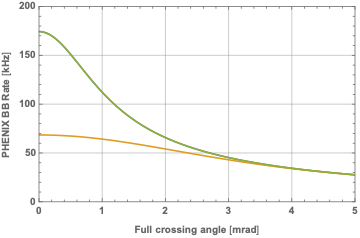
\includegraphics[width=0.7\linewidth]{figs/figure_cad1_prelim.png}  
    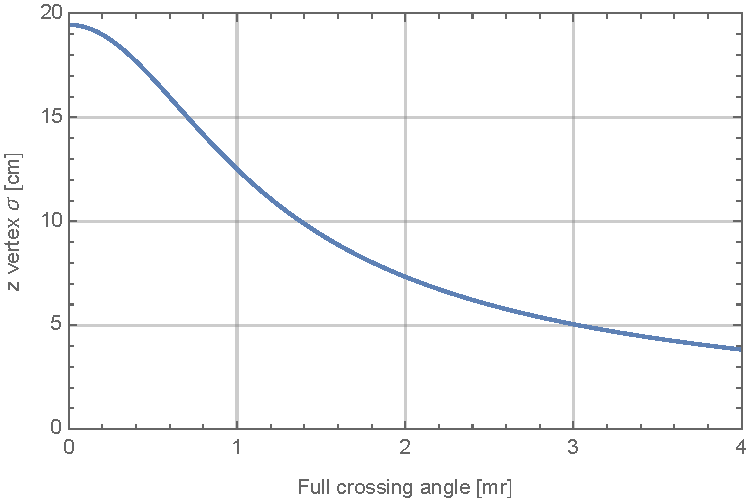
\includegraphics[width=0.62\linewidth]{figs/auau200-2023-202008131-z.pdf}
    \caption{C-AD {\textsc{Mathematica}} file generated \auau collision luminosity (left) and $z$-vertex Gaussian $\sigma$ (right) as a function of beam crossing angle.}
    \label{fig:mathauau1}
\end{figure}

\begin{figure}[h!]
    \centering
        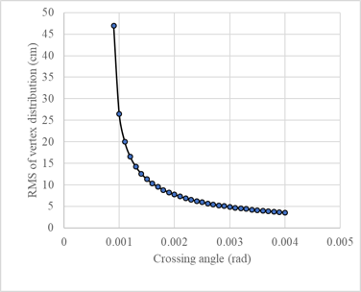
\includegraphics[width=0.7\linewidth]{figs/figure_cad2_prelim.png}  
    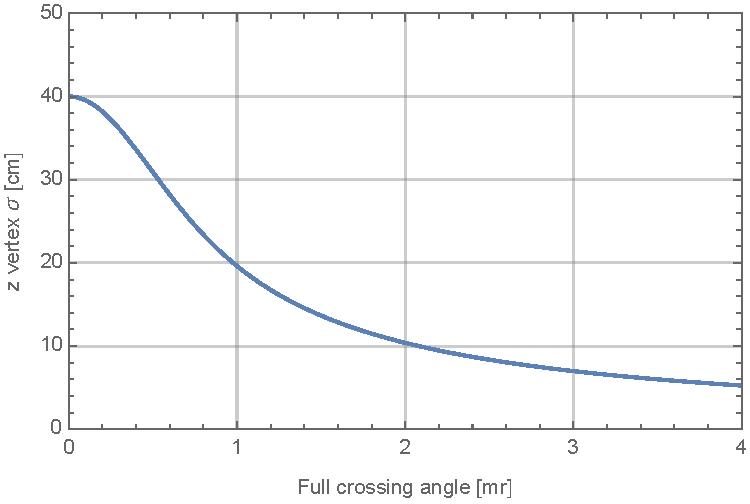
\includegraphics[width=0.62\linewidth]{figs/pp200-2023-202008131-z.pdf}
    \caption{C-AD {\textsc{Mathematica}} file generated \pp collision luminosity (left) and $z$-vertex Gaussian $\sigma$ (right) as a function of beam crossing angle.}
    \label{fig:mathpp1}
\end{figure}

\begin{figure}[h!]
    \centering
        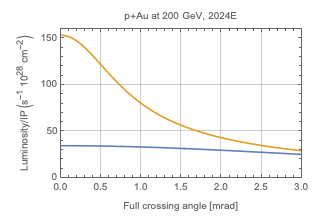
\includegraphics[width=0.7\linewidth]{figs/figure_cad3_prelim.png}  
    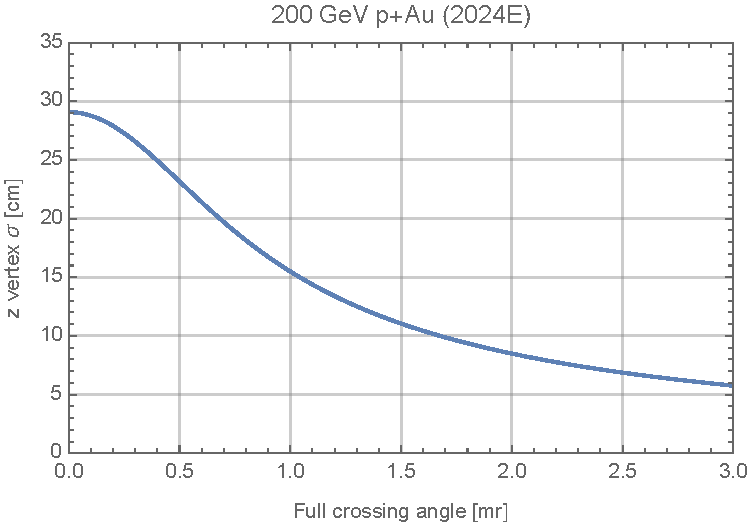
\includegraphics[width=0.62\linewidth]{figs/pau200-2024-z-202008190.pdf}
    \caption{C-AD {\textsc{Mathematica}} file generated \pau collision luminosity (left) and $z$-vertex Gaussian $\sigma$ (right) as a function of beam crossing angle.}
    \label{fig:mathpau1}
\end{figure}

